\documentclass[]{article}
\usepackage[spanish]{babel}
\usepackage{graphicx}
\usepackage[utf8]{inputenc}
\usepackage{fancyhdr}
\usepackage{lastpage}

\pagestyle{fancy}
\fancyhf{}
\rfoot{Page \thepage\hspace{1pt} de~\pageref{LastPage}}

\title{Practica 7}
\author{Guillermo Lopez Garcia}
\begin{document}
\maketitle

\textbf{Ejercicio 3.} \\

Respecto a este ejercicio, la conclusión es que la ejecución asincrona de
de las distintas hebras da como resultado una pequeña mejora respecto
a obtener el valor de variables locales a cada hebra.\\

Y por supuesto, da una gran mejora respecto a modificar un recurso compartido
con exclusión mutua. Es decir, modificar un recurso compartido activando
un cerrojo antes de modificar y desactivandolo después de salir de la sección
crítica. \\

\begin{figure}
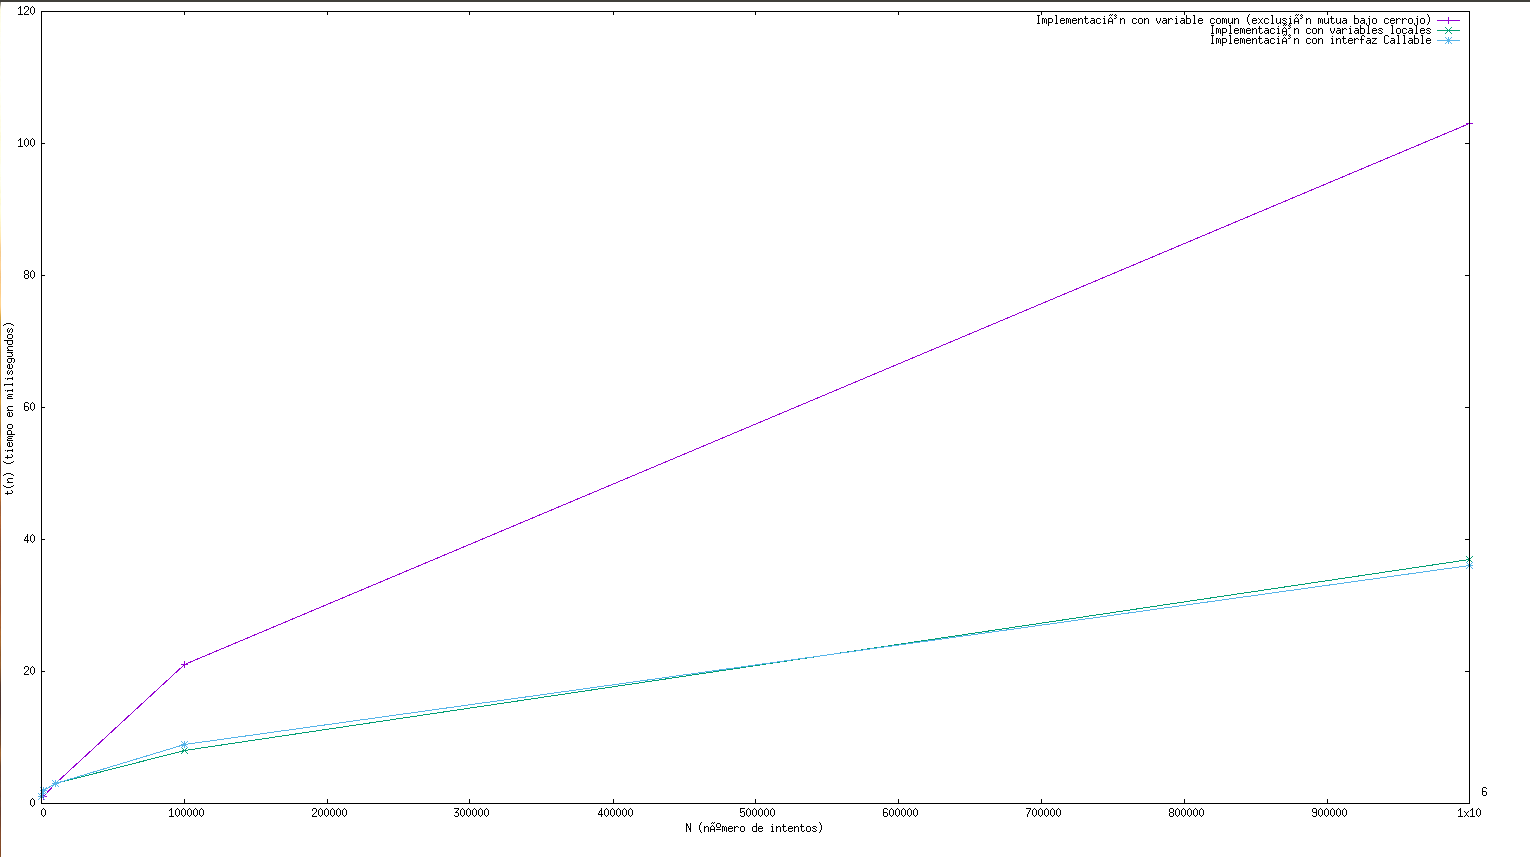
\includegraphics[width=\linewidth]{img.png}
\caption{Comparativa implementaciones concurrentes del método de montecarlo.}
\label{fig:comp}
\end{figure}

\end{document}
